We derive the Floquet-Fermi golden rule for our dressed quantum Hall system with the help of the $t$-$t'$ formalism. The $t$-$t'$-Floquet states \cite{grifoni98,wackerl20}
\begin{equation} \label{eq:c1}
  \ket{\psi_{n,m}(t,t')} =
  \exp(-\frac{i}{\hbar}\varepsilon_{n} t)\ket{\phi_{n,m}(t')},
\end{equation}
are derived by separating the aperiodic and periodic components of the Floquet states given in Eq.~(\ref{eq:14}). Additionally, these states fulfill the $t$-$t'$-Schrödinger equation \cite{grifoni98,wackerl20}
\begin{equation} \label{eq:c2}
  i \hbar \pdv{t}\ket{\psi_{n,m}(t,t')} =
  H_F(t') \ket{\psi_{n,m}(t,t')},
\end{equation}
where the \textit{Floquet Hamiltonian} defined as
\begin{equation} \label{eq:c3}
  H_F(t') =
  H_e(t') - i\hbar \pdv{t'}.
\end{equation}
Next, we can identify the time evolution operator corresponding to the $t$-$t'$-Schrödinger equation as
\begin{equation} \label{eq:c4}
  U_F(t,t_0;t') = \exp(-\frac{i}{\hbar}H_F(t')\left[t-t_0 \right]).
\end{equation}
The advantage of $t$-$t'$ formalism lies on this time evolution operator which avoids any time ordering operators \cite{wackerl20}.

We model the effect caused by impurities in the considered system as a single perturbation potential formed by a group of randomly distributed impurities.
Thus, we introduce a time-independent total perturbation $V(\vb{r})$ which has been turned on at the reference time $t=t_0$, and the $t$-$t'$-Schrödinger equation becomes
\begin{equation} \label{eq:c5}
  i \hbar \pdv{t}\ket{\Psi_{n,m}(t,t')} =
  \left[H_F(t') + V(\vb{r}) \right]\ket{\Psi_{n,m}(t,t')}.
\end{equation}
This introduces a new wave function solution $\ket{\Psi_{n,m}}$ for a system with a given perturbation. If $t\leq t_0$, both of the solutions for Eq.~(\ref{eq:c2}) and Eq.~(\ref{eq:c5}) coincide
\begin{equation} \label{eq:c6}
  \ket{\psi_{n,m}(t,t')} =\ket{\Psi_{n,m}(t,t')} \quad
  \text{when} \quad
  t \leq t_0.
\end{equation}
Next, we move our analysis into the interaction picture representation \cite{bruus04,mahan00} and in the interaction picture, we can identify the $t$-$t'$-Floquet state as
\begin{equation} \label{eq:c7}
  \ket{\Psi_{n,m}(t,t')}_I = U_0^{\dagger}(t,t_0;t')
  \ket{\Psi_{n,m}(t,t')}.
\end{equation}
Due to time-independence, the perturbation in the interaction picture has the same form as the Schrödinger picture representation
\begin{equation} \label{eq:c8}
  V_I(\vb{r}) = U_0^{\dagger}(t,t_0;t')V(\vb{r})U_0(t,t_0;t') =
  V(\vb{r}).
\end{equation}
This leads us to the $t$-$t'$-Schrödinger equation in the interaction picture representation
\begin{equation} \label{eq:c9}
  i \hbar \pdv{t}\ket{\Psi_{n,m}(t,t')}_I =
  V_I(\vb{r})\ket{\Psi_{n,m}(t,t')}_I,
\end{equation}
with the recursive solutions \cite{bruus04,mahan00}
\begin{equation} \label{eq:c10}
  \begin{aligned}
  \ket{\Psi_{n,m}(t,t')}_I = &\ket{\Psi_{n,m}(t_0,t')}_I \\
  &+
  \frac{1}{i\hbar}
  \int_{t_0}^t
  V_I(\vb{r}) \ket{\Psi_{n,m}(t_1,t')}_I dt_1.
  \end{aligned}
\end{equation}
Iterating the solution only up to the first order (Born approximation) we obtain
\begin{equation} \label{eq:c11}
  \begin{aligned}
    \ket{\Psi_{n,m}(t,t')}_I \approx &\ket{\psi_{n,m}(t_0,t')} \\
    &+
    \frac{1}{i\hbar}
    \int_{t_0}^t
    V_I(\vb{r}) \ket{\psi_{n,m}(t_0,t')} dt_1.
  \end{aligned}
\end{equation}

Since our $t$-$t'$-Floquet states create a basis, we can represent the solutions for the $t$-$t'$-Schrödinger equation given in Eq.~(\ref{eq:c5}) using our known $t$-$t'$-Floquet states as follows
\begin{equation} \label{eq:c12}
  \ket{\Psi_{\alpha}(t,t')} = \sum_{\beta} a_{\alpha,\beta}(t,t')
  \ket{\psi_{\beta}(t,t')}.
\end{equation}
Here, we used a single term notation to represent two quantum numbers; $\alpha \equiv (n_{\alpha},m_{\alpha})$ and $\beta \equiv (n_{\beta},m_{\beta})$.
Subsequently, we can identify the \textit{scattering amplitude} as $a_{\alpha,\beta}(t,t') =
\braket{\psi_{\beta}(t,t')}{\Psi_{\alpha}(t,t')}$ and we can evaluate this with
\begin{equation} \label{eq:c13}
  \begin{aligned}
  a_{\alpha,\beta}(t,t') = &
  \braket{\psi_{\beta}(t,t')}{\psi_{\alpha}(t,t')} \\
  &+
  \frac{1}{i\hbar}
  \int_{t_0}^t
  \bra{\psi_{\beta}(t_1,t')}
  V(\vb{r}) \ket{\psi_{\alpha}(t_1,t')} dt_1.
  \end{aligned}
\end{equation}
Since the $t$-$t'$-Floquet states are orthonormal and assuming $t_0 = 0$ and $\alpha \neq \beta$ this leads to
\begin{equation} \label{eq:c14}
  a_{\alpha,\beta}(t,t') =
  -
  \frac{i}{\hbar}
  \int_{0}^t
  \bra{\psi_{\beta}(t_1,t')}
  V(\vb{r}) \ket{\psi_{\alpha}(t_1,t')} dt_1.
\end{equation}

Next, we consider a scattering phenomenon when a electron scatters from a known $t$-$t'$-Floquet state $\ket{\psi_{\beta}(t,t')} $ into a distinct $t$-$t'$-Floquet state $\ket{\Psi_{\alpha}(t,t')}$ with a constant quansienergy $\varepsilon$ as follows
\begin{equation} \label{eq:c15}
  \begin{aligned}
  \ket{\psi_{\beta}(t,t')} &= \exp(-\frac{i}{\hbar}\varepsilon_{\beta} t)
  \ket{\phi_{\beta}(t')} \\
  &
  \xRightarrow{\text{scattering}}
  \ket{\Psi_{\alpha}(t,t')} = \exp(-\frac{i}{\hbar}\varepsilon t)
  \ket{\Phi_{\alpha}(t')}.
  \end{aligned}
\end{equation}
\begin{figure}[b]
  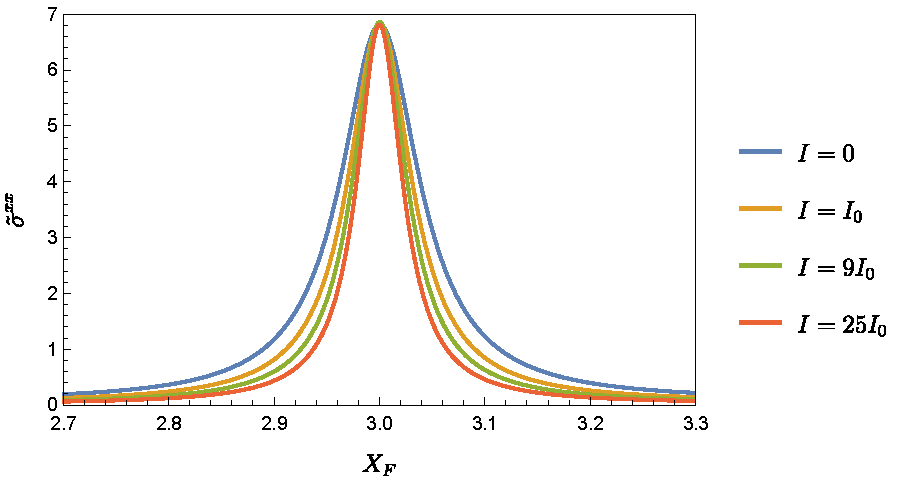
\includegraphics[scale=1.0]{figures/fig_6.pdf}
  \caption{Scattering from known $\ket{\psi_{\beta}(t,t')}$ state to a constant energy state $\ket{\Psi_{\alpha}(t,t')}$ due to the scattering potential created by impurities in the material.}
  \label{fig:2}
\end{figure}
This phenomenon is illustrated in Fig.~\ref{fig:2}.
We can calculate the scattering amplitude for this scattering scenario using the expression derived in Eq.~(\ref{eq:c14}) as follows
\begin{equation} \label{eq:c16}
  \begin{aligned}
    a_{\alpha\beta}(t,t') =
    -\frac{i}{\hbar}
    \int_{0}^t
    e^{\frac{i}{\hbar}\left(\varepsilon_{\beta} - \varepsilon \right)t_1}
    \bra{\phi_{\beta}(t')}
    V(\vb{r}) \ket{\phi_{\alpha}(t')}  dt_1.
  \end{aligned}
\end{equation}
By assuming for a long duration ($t \rightarrow \infty$), we can turn this integral into a delta distribution
\begin{equation} \label{eq:c17}
  \begin{aligned}
    a_{\alpha\beta}(t') =
    -2\pi i \delta(\varepsilon_{\beta} - \varepsilon)Q,
  \end{aligned}
\end{equation}
where $Q = \bra{\phi_{\beta}(t')} V(\vb{r}) \ket{\phi_{\alpha}(t')}$ and using the completeness properties we can re-write this as
\begin{equation} \label{eq:c18}
    Q =
    \sum_{\vb{k}}\sum_{\vb{k'}}
    \braket{\phi_{\beta}(t')}{\vb{k'}}
    \mel{\vb{k'}}{V(\vb{r})}{\vb{k}}
    \braket{\vb{k}}{\phi_{\alpha}(t')}.
\end{equation}
Moreover, separating $x$-directional and $y$-directional momentum components, we can simply this to obtain
\begin{equation} \label{eq:c19}
    Q =
    \sum_{k_x}\sum_{{k'}_x}
    \int_{-\infty}^{\infty} \int_{-\infty}^{\infty}
    V_{\vb{k'},\vb{k}}
    \phi_{\beta}^{\dagger}(\vb{k'},t')
    \phi_{\alpha}(\vb{k},t')  dk_y d{k'}_y,
\end{equation}
with $V_{\vb{k'},\vb{k}} = \mel{\vb{k'}}{V(\vb{r})}{\vb{k}}$.

Since we are presenting the the perturbation potential $V(\vb{r})$ by a group of randomly distributed impurities, we take into account $N_{imp}$ number of identical single impurity potentials distributed at randomly but in fixed positions $\vb{r}_i$. Thus, we can describe the scattering potential $V(\vb{r})$ as the sum of uncorrelated single impurity potentials $\upsilon(\vb{r})$
\begin{equation} \label{eq:c20}
  V(\vb{r}) =
  \sum_{i=1}^{N_{imp}}
  \upsilon (\vb{r}-\vb{r}_i).
\end{equation}
Furthermore, we model the perturbation $V(\vb{r})$ as a Gaussian random potential where one can choose the zero of energy such that the potential is zero on average. This model is characterized by the following two equations \cite{akkermans10}
\begin{subequations}
\begin{equation} \label{eq:c21a}
  \expval{\upsilon(\vb{r})}_{imp} =0,
\end{equation}
\begin{equation} \label{eq:c21b}
  \expval{\upsilon(\vb{r})\upsilon(\vb{r'})}_{imp} = \Upsilon(\vb{r}-\vb{r'}),
\end{equation}
\end{subequations}
where $\expval{\cdot}_{imp}$ represents the average over the impurity disorder and $\Upsilon(\vb{r}-\vb{r'})$ is any decaying function depends only on $\vb{r}-\vb{r'}$. In addition, this model assumes that $\upsilon (\vb{r}-\vb{r'})$ only depends on the magnitude of the position difference $|\vb{r}-\vb{r'}|$, and it decays with a characteristic length $r_c$. Since this study considers the case where the wavelength of radiation or scattering electron is much greater than $r_c$, it is a better approximation to make two-point correlation function to be
\begin{equation} \label{eq:c22}
  \expval{\upsilon(\vb{r})\upsilon(\vb{r'})}_{imp} = \Upsilon_{imp}^2\delta(\vb{r}-\vb{r'}),
\end{equation}
where $\Upsilon_{imp}^2$ is a constant. A random potential $V(\vb{r})$ with this property is called white noise \cite{akkermans10}. Then we can approximately model the total scattering potential as
\begin{equation} \label{eq:c23}
  V(\vb{r}) =
  \sum_{i=1}^{N_{imp}}
  \Upsilon_{imp} \delta(\vb{r}-\vb{r}_i).
\end{equation}
Here we can identify the $\Upsilon_{imp}$ as the strength of the delta potential.
Furthermore, we can calculate $V_{\vb{k'},\vb{k}}$ using this assumption as follows
\begin{subequations} \label{eq:c24}
\begin{align}
 V_{\vb{k'},\vb{k}} & =
 \mel**{\vb{k'}}{\sum_{i=1}^{N_{imp}}
 \Upsilon_{imp} \delta(\vb{r}-\vb{r}_i)}{\vb{k}} \label{eq:c24a} \\
 & =
 \sum_{i=1}^{N_{imp}}
 \int_{-\infty}^{\infty} \left[
 \frac{1}{\sqrt{L_xL_y}} e^{ik'_y y} \delta(y-y_i) \nonumber \right. \\
 & \left. \qquad\quad\times
 \frac{1}{\sqrt{L_xL_y}} e^{-i{k}_y y}
 \mel**{k'_x}{\Upsilon_{imp} \delta(x-x_i)}{k_x} \right] dy \label{eq:c24b} \\
  & =
 \sum_{i=1}^{N_{imp}} \frac{1}{{L_xL_y}}
 e^{i(k'_y - k_y )y}
 \mel**{k'_x}{\Upsilon_{imp} \delta(x-x_i)}{k_x} \label{eq:c24c}.
\end{align}
\end{subequations}
Since $\upsilon (\vb{r})$ in momentum space is a constant value, each impurity  produce same impurity potential for every $x$-directional momentum pairs. Additionally, assuming the total number of scatters $N_{imp}$ is microscopically large, we can derive
\begin{subequations} \label{eq:c25}
  \begin{align}
    V_{\vb{k'},\vb{k}}
    & =
    V_{k'_x,k_x}
    \frac{N_{imp}}{L_y L_x} \int_{-\infty}^{\infty}
    e^{i\left({k'}_y - k_y \right)y_i} dy_i \label{eq:c25a} \\
    & =
    \eta_{imp} V_{k'_x,k_x} \delta(k'_y - k_y). \label{eq:c25b}
  \end{align}
\end{subequations}
In the above equation we introduced
\begin{equation} \label{eq:c26}
  V_{{k'}_x,k_x} =
  \mel**{k'_x}{\Upsilon_{imp} \delta(x-x_i)}{k_x},
\end{equation}
which is a constant value for every $i$-th impurity. Moreover, $\eta_{imp}$ is the number of impurities in a unit area. It is important to note that in the above expression $\braket{x}{k_x} = e^{-ik_xx}$.

Now using Eq.~(\ref{eq:10}) and Eq.~(\ref{eq:c25b}) on Eq.~(\ref{eq:c19}), we obtain
\begin{equation} \label{eq:c27}
  \begin{aligned}
    Q  =
    \sum_{k_x}\sum_{{k'}_x} &
    {\eta_{imp} V_{{k'}_x,k_x}} L_x
    \int_{-\infty}^{\infty} \int_{-\infty}^{\infty}
    \delta({k'}_y - k_y)
    \\
    & \times
    \widetilde{\chi}_{n_{\beta}} \bm{\left(} {k'}_y -b\cos(\omega t) \bm{\right)}
    \widetilde{\chi}_{n_{\alpha}}  \bm{\left(}k_y -b\cos(\omega t) \bm{\right)}
    \\
    & \times
    e^{i[{k'}_y - k_y]d\sin(\omega t)}
    e^{i[{k'}_y {y'}_0 - k_y y_0]}
     dk'_y dk_y.
  \end{aligned}
\end{equation}
Here we have changed the time variable $t' \rightarrow t$ only for the simplicity of notation. We can more simply this as
\begin{equation} \label{eq:c28}
  \begin{aligned}
    Q =
    \sum_{k_x}\sum_{{k'}_x} \eta_{imp} L_x V_{{k'}_x,k_x} I,
  \end{aligned}
\end{equation}
with
\begin{equation} \label{eq:c29}
  \begin{aligned}
    I =
    \int_{-\infty}^{\infty}
    \widetilde{\chi}_{n_{\beta}} &\bm{\left(}  k_y -b\cos(\omega t) \bm{\right)}
    \widetilde{\chi}_{n_{\alpha}} \bm{\left(} k_y -b\cos(\omega t) \bm{\right)} \\
    & \times
    \exp \bm{(}
      -ik_y  \left(y_0 - {y'}_0 \right)
    \bm{)} dk_y.
  \end{aligned}
\end{equation}
To avoid the energy exchange from the dressing field and electrons in Landau levels, the applied radiation must be a purely dressing field.
Therefore, in this study we assume that the dressing field can only renormalize the the probability of electron scattering inside a same Landau energy level $(n_{\alpha} = n_{\beta} =N)$. This transform the Eq.~(\ref{eq:c29}) to
\begin{equation} \label{eq:c30}
    I =
    \int_{-\infty}^{\infty}
    \widetilde{\chi}_N^2 \bm{\left(}  k_y -b\cos(\omega t) \bm{\right)}
    \exp \bm{(}
      -ik_y  \left(y_0 - {y'}_0 \right)
    \bm{)} dk_y.
\end{equation}
Using the Fourier transform of Gauss-Hermite functions \cite{celeghini21} and the convolution theorem \cite{arfken85,bracewell78} we obtain
\begin{equation} \label{eq:c31}
  \begin{aligned}
    I =
    {2\pi} &
    \exp \bm{(} b({y'}_0 - y_0)\cos(\omega t) \bm{)} \\
    & \times
    \int_{-\infty}^{\infty}
    {\chi}_{N}(y)
    {\chi}_{N}(y_0 - {y'}_0 - y) dy.
  \end{aligned}
\end{equation}
Finally, we can evaluate the scattering amplitude derived in Eq.~(\ref{eq:c17}) for given $k_x = 2\pi m_{\alpha}/L_x$ and $k'_x =  2\pi m_{\beta}/L_x$ as follows
\begin{equation} \label{eq:c32}
  \begin{aligned}
    a_{\alpha\beta}&(k_x,k'_x,t)
    \\
    & =
    -2\pi i
    \eta_{imp} L_x V_{{k'}_x,k_x}
    e^{ b({y'}_0 - y_0)\cos(\omega t)}\\
    & \quad\times
    \delta(\varepsilon_{N} - \varepsilon)
    \int_{-\infty}^{\infty}
    {\chi}_{N}(y)
    {\chi}_{N}(y_0 - {y'}_0 - y) dy.
  \end{aligned}
\end{equation}
Since this scattering amplitude is time-periodic, we can write this as a Fourier series expansion
\begin{equation} \label{eq:c33}
    a_{\alpha\beta}(k_x,k'_x,t) =
    \sum_{l=-\infty}^{\infty} a^l_{\alpha\beta}(k_x,k'_x) e^{-il\omega t}.
\end{equation}
In addition, using Jacobi-Anger expansion \cite{cuyt08,abramowitz64}
\begin{equation} \label{eq:c34}
    e^{iz\cos(\theta)} = \sum_{l=-\infty}^{\infty} i^l J_l(z) e^{-il\theta},
\end{equation}
where $J_l(\cdot)$ are Bessel functions of the first kind with $l$-th integer order, we can re-write the Eq.~(\ref{eq:c32}) as follows
\begin{equation} \label{eq:c35}
  \begin{aligned}
    a_{\alpha\beta}&(k_x,k'_x,t)  \\
    & =
    \sum_{l=-\infty}^{\infty}
    -2\pi i^{l+1}
    \eta_{imp} L_x V_{{k'}_x,k_x}
    J_l\bm{(}b({y'}_0 - y_0)\bm{)} \\
    & \quad\times
    \delta(\varepsilon_{N} - \varepsilon)
    \int_{-\infty}^{\infty}
    {\chi}_{N}(y)
    {\chi}_{N}(y_0 - {y'}_0 - y)  dy \;e^{-il\omega t}.
  \end{aligned}
\end{equation}
Thus, we can identify the Fourier series component of the scattering amplitude as
\begin{equation} \label{eq:c36}
  \begin{aligned}
    a^l_{\alpha\beta}(k_x,k'_x) = &
    -2\pi i^{l+1}
    \eta_{imp} L_x V_{{k'}_x,k_x}\\
    & \times
    \delta(\varepsilon_{N} - \varepsilon)
    J_l\bm{(}b({y'}_0 - y_0)\bm{)}\\
    & \times
    \int_{-\infty}^{\infty}
    {\chi}_N(y)
    {\chi}_N(y_0 - {y'}_0 - y) dy.
  \end{aligned}
\end{equation}
Furthermore, we can define \textit{transition probability matrix} as
\begin{equation} \label{eq:c37}
    \left(A_{\alpha\beta} \right)^{l,l'} =
    a^l_{\alpha\beta}\left[a^{l'}_{\alpha\beta} \right]^{*},
\end{equation}
and this becomes
\begin{equation} \label{eq:c38}
  \begin{aligned}
      \left(A_{\alpha\beta} \right)^{l,l'}(k_x,k'_x) = &
      \left({ 2 \pi \eta_{imp} L_x V_{{k'}_x,k_x}}\right)^2
      \delta^2(\varepsilon_{N} - \varepsilon) \\
      & \times
      J_l\bm{(}b({y'}_0 - y_0)\bm{)} J_{l'}\bm{(}b({y'}_0 - y_0)\bm{)}\\
      & \times
      \left|
      \int_{-\infty}^{\infty}
      {\chi}_N(y)
      {\chi}_N(y_0 - {y'}_0 - y) dy \right|^2.
  \end{aligned}
\end{equation}
Then describing the square of the delta distribution using the following interpretation \cite{dini16,kibis14}
\begin{equation} \label{eq:c39}
    \delta^2(\varepsilon) =
    \delta(\varepsilon)\delta(0) =
    \frac{\delta(\varepsilon)}{2\pi \hbar}
    \int_{-t/2}^{t/2} e^{i0\times t'/\hbar} dt'\; =
    \frac{\delta(\varepsilon)t}{2\pi \hbar},
\end{equation}
and executing the time derivation operation on each matrix element of transition probability matrix, we receive the \textit{transition amplitude matrix} elements
\begin{equation} \label{eq:40}
  \begin{aligned}
    \Gamma_{\alpha\beta}^{ll'}(k_x,k'_x) = &
    \frac { 2\pi \eta_{imp}^2 L_x^2}{ \hbar} |V_{{k'}_x,k_x}|^2
    \delta(\varepsilon_{\beta} - \varepsilon)\\
    & \times
    J_l\bm{(}b({y'}_0 - y_0)\bm{)} J_{l'}\bm{(}b({y'}_0 - y_0)\bm{)} \\
    & \times
    \left|
    \int_{-\infty}^{\infty}
    {\chi}_N(y)
    {\chi}_N(y_0 - {y'}_0 - y) dy \right|^2.
  \end{aligned}
\end{equation}

Additionally, the inverse scattering time matrix can be identified as the sum of all available momentum over the impurity averaged transition probability matrix element \cite{wackerl20,wackerlthesis20}
\begin{equation} \label{eq:41}
    \left(\frac{1}{\tau(\varepsilon,k_x)} \right)^{ll'}_{\alpha\beta} =
    \frac{1}{L_x} \sum_{{k'}_x}
    \expval**{\Gamma_{\alpha\beta}^{ll'}({k'}_x,k_x)}_{imp}.
\end{equation}
Next, applying the 1-dimensional momentum continuum limit $\sum_{{k'}_x} \longrightarrow {L_x}/{2\pi}\int d {k'}_x$, we can obtain
\begin{widetext}
\begin{equation} \label{eq:42}
  \begin{aligned}
    \left(\frac{1}{\tau(\varepsilon,k_x)}\right)^{ll'}_{\alpha\beta} = &
    \frac { 2\pi \eta_{imp}^2 L_x^2}{ \hbar}
    \frac{V_{imp}}{2\pi}
    \delta(\varepsilon_{\beta} - \varepsilon) \\
    & \times
    \int_{-\infty}^{\infty} \left\{
    J_l\bm{\left(}\frac{b\hbar}{eB}({k}_x - {k'}_x)\bm{\right)}
    J_{l'}\bm{\left(}\frac{b\hbar}{eB}({k}_x - {k'}_x)\bm{\right)}
    \left|
    \int_{-\infty}^{\infty}
    {\chi}_N(y)
    {\chi}_N \bm{\left(}\frac{\hbar}{eB} ({k'}_x - {k}_x) - y \bm{\right)} dy\right|^2 \right\} d {k'}_x.
  \end{aligned}
\end{equation}
Here an impurity average of white noise potential allows to identify $\expval{|V_{{k'}_x,k_x}|^2}_{imp} = V_{imp}$.
Finally, using substitutions $k'_x = k_1$ and $y = \flatfrac{\hbar{k_2}}{(eB)}$, we can derive our expression for the inverse scattering time matrix for $N$-th Landau
level as follows
\begin{equation} \label{eq:43}
  \begin{aligned}
    \left(\frac{1}{\tau(\varepsilon,k_x)}\right)^{ll'}_{N} &=
    \frac { \eta_{imp}^2 L_x^2 \hbar V_{imp}}{e^2B^2}
    \delta(\varepsilon - \varepsilon_{N}) \\
    & \times
    \int_{-\infty}^{\infty} \left\{
    J_l\bm{\left(}\frac{b\hbar}{eB}({k}_x - k_1)\bm{\right)}
    J_{l'}\bm{\left(}\frac{b\hbar}{eB}({k}_x - k_1)\bm{\right)}
    \left|
    \int_{-\infty}^{\infty}
    {\chi}_N\left(\frac{\hbar}{eB}k_2 \right)
    {\chi}_N \bm{\left(}\frac{\hbar}{eB} (k_1 - k_x - k_2) \bm{\right)} dk_2 \right|^2 \right\} d k_1.
  \end{aligned}
\end{equation}
\end{widetext}
